\section{Algorithmus} % High-level description

% Idee für Layout: 
% - Gruppenelemente in Blase passen
% - festes Layout pro Hierarchiestufe berechnen
% - Layouts in Gruppen richten sich nach Ports aus Layout von Stufe darüber
% - Layouts niedrigerer Stufe beeinflussen Layouts höherer Stufe nur durch benötigten Platz


% was betrachten? problem wie oben definiert -> hier unser Ansatz
Für das oben definierte Layoutproblem haben wir uns einen Lösungsansatz überlegt.
% was für design/layout-entscheidungen?
Die wichtigste Designentscheidung und damit Grundiee des Layouts ist es, jede Gruppen in einen Kreise zu packen und Kanten über Gruppengrenzen nur über feste Ports zu führen.
Dadurch werden die Layouts pro hierarchische Stufe und Gruppe getrennt. 
Ist ein Layout einer höhere Stufe berechnet, hat dies nur durch das Festlegen der Portpositionen Einfluss auf das Layout von Gruppen eine Stufe tiefer.  Layouts von niedrigeren Stufen beieinflussen übergeordnete Layouts nur durch ihren benötigten Platz.
Grafik \ref{f:Layoutbeispiel} zeigt so ein Layout.
Außerdem können Gruppen geöffnet oder geschlossen dargestellt werden. 
Hierbei haben wir besonders darauf geachtet, dass beim Öffnen oder Schließen einer Gruppe das Gesamtlayout der Karte nur wenig verändert wird.


\begin{figure}[h!]
\begin{center} 
  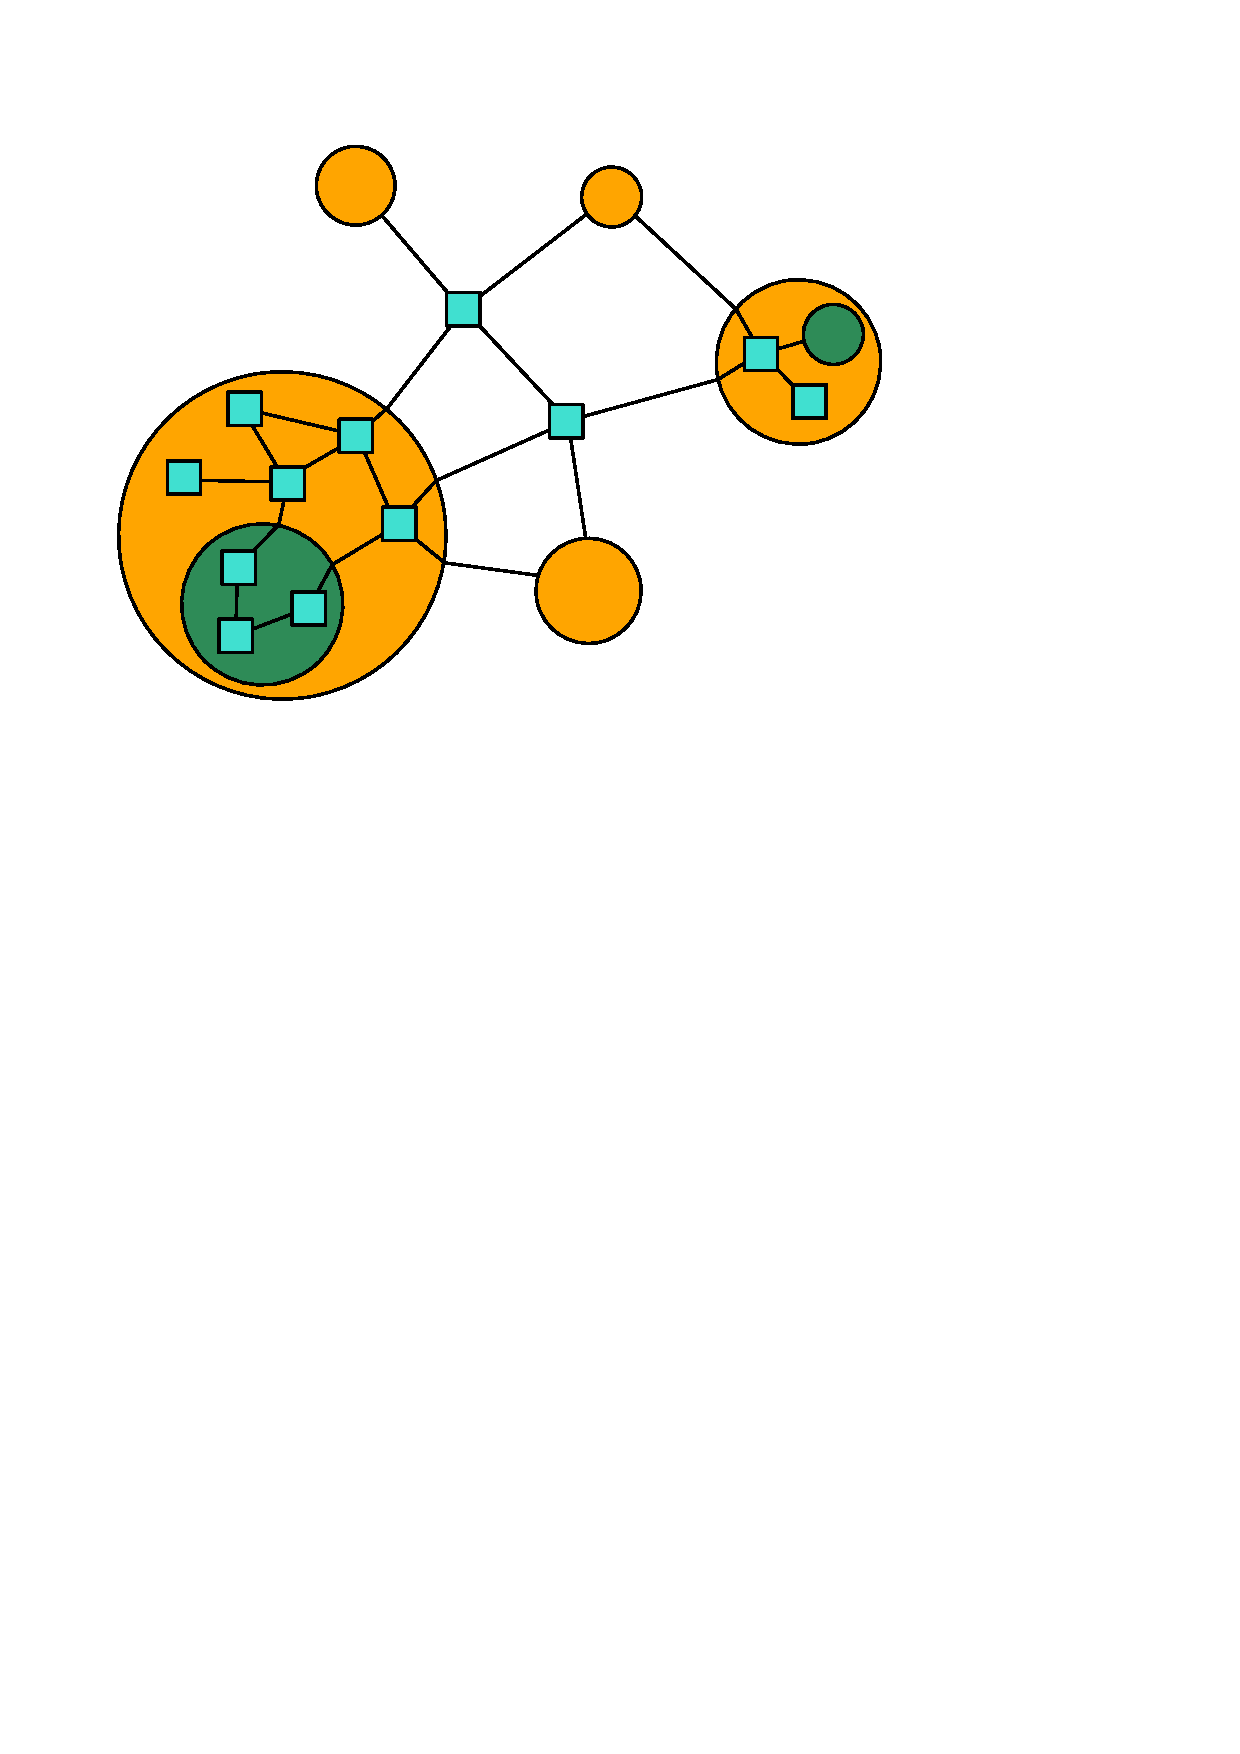
\includegraphics{Pics/Layoutbeispiel.pdf}
  \caption{Beispiellayout einer abstrahierten Argumentkarte nach unserem Konzept.}
  \label{f:Layoutbeispiel}
\end{center}
\end{figure}

% welche Schritte?
Im Folgenden beschreiben wir einen Algorithmus um so ein Layout zu berechnen, 
sowie das Konzept um Layoutänderungen beim Öffnen oder Schließen von Gruppen gering zu halten.
Zunächst widmen wir uns jedoch den Gruppengrößen. 


\subsubsection*{Kräftebasierte Algorithmen}

% verwendete Kräftebasierte Algorithmen
\todo[inline]{Kräftebasierte Algorithmen angeben, siehe zB Paper in bibtex}




% Größe geschlossener Gruppen
\subsubsection*{Gruppengrößen}
\todo[inline]{Spezifiziere Gruppengroessen}


% DEFINITION Anker 
% Pseudoknoten, wird nicht gerendert % hat Kanten zu allen Knoten, welche er Ankert  % optimale Kantenlänge = 0  % Federkraft Fallabhängig und jeweils zu spezifizieren
\subsubsection*{Anker}
Da wir in der genaueren Beschreibung des Algorithmus öfters sogenannte \textit{Anker} verwenden werden, wollen wir diese kurz definieren. 
Ein Anker für einen Knoten ist ein Pseudoknoten, ein Ankerpunkt, welcher also nich gerendert wird, sowie eine Kante zu diesem Knoten. 
Anders als normale Kanten ist die optimale Kantenlänge eines Ankers  0. Außerdem hat sein Ankerpunkt  eine feste Position im Layout. 
In einem kräftebasierten Algorithmus wirkt der Anker auf seinen Knoten nun wie eine weitere Feder, die ihn zum Ankerpunkt hinzieht.
Die Kraft der Feder kann wie eine normale Kante gehandhabt werden oder bei Bedarf auch anders spezifiziert werden.
%\todo[inline]{Grafik Anker (?)}


\subsection{Konzept und Idee}
% Weitere Constraints für Layout
% Resultat: alle Gruppen geschlossen, jedoch Layout pro Gruppe mit geschlossenen/geöffneten Kind-Gruppen bekannt
Wenn alle Gruppen beim Öffnen einer Karte geschlossen sind, sollte es auf großen Karten einfach sein direkt einen Überblick gewinnen zu können.
Deshalb liefert der folgendes Algorithmus ein Layout bei dem alle Gruppen geschlossen sind.

Unser Layoutalgorithmus, grob beschrieben in Algorithmus \ref{Layoutalgorithmus}, ist in 2 Phasen unterteilt. 
In der ersten Phase, Zeilen 1 -8, werden die in einem bottem-up Ansatz die Größen der Gruppen berechnet. 
Dies beginnt auf der tiefsten Stufe und geht dann iterativ nach oben, da die Größe einer Gruppe jeweils für die Größe der übergordneten Gruppe bzw obersten Stufe notwendig ist.
In einem top-down Ansatz wird in der zweiten Phase, Zeilen 9-17, werden nun die Layouts pro Stufe berechnet und die Ports festgelegt. 


\begin{algorithm}[H]
\label{Layoutalgorithmus}
\SetAlgoLined
\Ein{Graph $G=(V,E)$ mit Gruppen $S$ } % mit Koten $V$ mit Größe, gerichteten \& gefärbten Kanten $E$, Mengen $S$ von Knoten und Elementen aus $S$
\Aus{Gruppen-hierarchisches Layout von $G$ } % mit diesen und jenen Eigenschaften, evtl Name einführen für Referenzierung
$i = $ niedrigste Stufe einer Gruppe \;
\Solange{$i \geq 0$}{ % benötigt, dass oberste Ebene auch Gruppe
  \Fuer{Jede Gruppe $H$ auf Stufe $i$} {
	berechnete Layout $\L'_H$ der Gruppe $H$\;
	berechne benötigte Fläche des Gruppenlayouts\;	
  }
  $i= i + 1$\;
}
Lege Ports für Gruppen auf Stufe 1 fest\;
$i = Anzahl Stufen$\;
\Solange{$i \leq$ Anzahl Stufen}{ % benötigt, dass oberste Ebene auch Gruppe
  \Fuer{Jede Gruppe $H$ auf Stufe $i$} {
	berechnete Layout $\L_H$ der Gruppe $H$ unter Berücksichtigung der Ports\;
	Lege Ports für Gruppen in $H$ auf Stufe $i - 1$ fest;
  }
  $i= i - 1$\;
}
\caption{Layoutalgorithmus}
\end{algorithm}


\subsubsection{Bottom-up Anteil des Algorithmus}
% Layoutberechnung
		% bottom-up und top-down
	% (Layoutalgorithmus hierbei egtl frei wählbar, kräftebasiert aber besser in Hinsicht auf Verhalten Algorithmus mit Ankern)
	% bottom-up
		% Berechne Layouts pro Gruppe auf niederigster Stufe
		% versuche hierbei Fläche klein zu halten bzw Elemente in Kreis zu zwingen
		% Berechne die approximierte resultierende benötigte Fläche für Gruppe
		% Benutze appr. benötigte Fläche für Wiederholung des Schritts auf Stufe höher (bis auf letzte)
Schauen wir uns den bottom-up Teil des Algorithmus genauer an. Ziel ist es zunächst für jede Gruppe ein benötigte Größe zu approximieren.
Da für die Gruppen der Positionen die Positionen der Ports jedoch noch nicht bekannt sind, werden die Gruppen zunächst ohne Ports gelayoutet.
Hierfür kann einer der oben genannten kräftebasierten Algorithmen verwendet werden. 
Zusätzlich wird jedoch für jeden Knoten noch ein Anker zu einer relativen Mitte der Gruppe gesetzt. 
Auf Grund der Verwendung eines kräftebasierten Algorithmus hält dies die Gruppe, die nicht zwingend eine Zusammenhangskomponente sein muss, zusammen 
und konzentriert sie einem eher kreisförmigen Bereich. Anderenfalls könnte sich zum Beispiel eine lange Kette bilden.
Da die Größe von Kindgruppen einer Elterngruppe für deren Layout benötigt wird, beginnt der Algorithmus auf der tiefsten Stufe,
also bei den Gruppen, die in den meisten Gruppen enthalten sind. Wurde ein Layout berechnet, kann ein Kreis darum gelegt werden und somit die Größe approximiert werden.
Mit der oben genannten Rechnung für die Größe von geschlossenen Gruppen, kann nun also die Größe für das Layout eine Stufe höher verwendet werden.
Dies wiederholt sich bis zur obersten Stufe. Hier sind jedoch kein Anker zu einem Mittelpunkt mehr zwingend nötig. 
Außer man möchte die gesamte Karte eventuell in einen keisförmigen Bereich ziehen.


\todo[inline]{Grafik bottom-up und dadurch mehr Details in Text}

\subsubsection{Top-down Anteil des Algorithmus}
Der Übergang vom bottom-up zum top-down Anteil erfolgt, wenn auf der obersten Stufe das Layout berechnet wird. 
Wenn zu Beginn, wie bei uns gewählt, alle Gruppen geschlossen sind, dann ist dieses berechnete Layout auch das Layout, dass beim öffnen der Karte zu sehen ist.
Auf der obersten Stufe beginnend und durch das berechnete Layout vorgegeben, legen wir nun die Ports der Gruppen nächste-niedrigen Stufe fest und berechnen deren Layout.
Wie ein Layout für eine Guppe berechnet wird und die Ports festgelegt werden, erläutern wir im folgenden genauer. 
	% top-down
		% berechne Layout auf oberster Stufe
		% Lege Ports für Gruppen auf oberster Stufe fest
		
		% berechne iterativ absteigend Layouts in Gruppen mit festgelegten Ports
\todo[inline]{Grafik top-down}



\todo[inline]{FRAGE: Hier anmerken, dass Prozess wiederholt werden könnte? (hoch runter hoch runter) Oder eher weiter unten?}




\subsubsection{Layout in Gruppen in Abhängigkeit von Ports}
% Problem: Layout eines Graphens (mit Labelknoten) innerhalb eines Kreises mit Ports für ausgehende kanten
% Äquivalent: Layout eines Graphens mit punktförmigen Knoten auf Kreis und gelabelten Knoten innerhalb des Kreises

% was betrachten?
In diesem Abschnitt betrachten wir Zeile 13 des Layoutalgorithmus \ref{Layoutalgorithmus} genauer. 
% was ist ziel?
Hier ist das Ziel ein Layout für eine Gruppe mit bereits gegebenen Ports, also mit gegebenen Winkel für Kanten zur Gruppe, zu finden.
Das heißt, wir suchen nun einen Layout für den durch die Gruppe induzierten Teilgraphen sowie aus der Gruppe herausgehende Kanten.
Dieses soll, wie oben beschrieben, ein Layout innerhalb eines Kreises sein und die Gruppengrenze-überschreitenden Kanten zu den festgelegten Ports führen.
% was ist schwierig?
Eine der Herausforderung hierbei ist, eine geeignete Größe für den Kreis um die Gruppe zu finden. Auch zum finden dieses Layouts benutzen wir wieder einen kräftebasierten Algorithmus.

% Bemerkung: Layout in einer Gruppe ist von Layouts in anderen Stufen und Gruppen unabhängig (außer durch Ports)

		%// Genau zu spezifizieren:
		%// - wie wird es modelliert: Ports als feste Knoten? nur Reihenfolge festlegen und flexibel auf gewissem Radius? ..
		%// Ports bleiben fest. Argument: Sowieso Winkel an Ports, nich wesentliche Winkel-Änderung erwartet bei Veränderung
% was ist gegeben?
% wie betrachten wir es? wie ist es modeliert?
Gegeben sei nun also eine Gruppe $H$. Vom Layouts der nächsthöheren Stufe wurden bereits die Ports der Gruppe festgelegt, d.h. wir haben die Winkel an denen Gruppengrenze-überschreitenden Kanten den Kreis schneiden sollen. Diese Ports modellieren wir als feste Knoten auf dem Kreis der Gruppe an ihren jeweiligen Winkeln.
Des weiteren haben wir bereits ein Layout $\mathcal{L_H}$ der Gruppe $H$ ohne Gruppengrenze-überschreitenden Kanten in Zeile 4 des Layoutalgorithmus \ref{Layoutalgorithmus}  berechnet.
Aus Zeile 5 haben wir daher auch eine erste Größe für den Kreis der Gruppe, welche durch den Radius beschreiben und durch $R'_H$ gegeben sei. 
% was sind die essentiellen punkte?
	% anfangslayout, anfangsradius, neuer radius, 
Der grobe Ablauf des Algorithmus ist in Algorithmus \ref{Gruppenlayoutalgorithmus} beschrieben. 
Die essentiellen Schritte sind also die Wahl eines Anfangslayouts (Zeile 1), Finden eines optimalen Radius (2) und das Berechnen eines Layouts (3).

\begin{algorithm}[H]
\label{Gruppenlayoutalgorithmus}
\SetAlgoLined
\Ein{Gruppe $H$, sowie Ports und Kanten zu Ports} 
\Aus{Gruppenlayout $\L_H$ von $H$ }
Wähle Anfangslayout\;
Finde Radius $R$ für Kreis\;
Berechne Gruppenlayout  $\L_H$ mit kräftebasiertem Algorithmus\;
\caption{Gruppenlayoutalgorithmus}
\end{algorithm}



Die Wahl eines Anfangslayouts und das finden eines optimalen Radius beschrieben wir  in den folgenen Abschnitten  genauer. 
% - Anziehung zu Mittelpunkt
	% ja, mit Kanter
	% schwache Feder mit Faktor $\alpha$
Für die Berechnung eines Gruppenlayouts verweisen wir wieder lediglich auf die oben genannten kräftebasierten Algorithmen, welche mit Knoten von bestimmter Größer umgehen können. 
Jedoch schlagen wir auch hier wieder das hinzunehmen eines Ankers vor, welcher alle Elemente zur Mitte des Kreises ziehen soll.
 Dies soll auch verhindern, dass eventuell nicht zusammenhängde Komponenten der Gruppe auseinander driften. Die Kraft dieses Ankers sei mit dem Faktor $\alpha$ beschrieben. 

% - Anfangslayout: 
\subparagraph{Anfangslayout}

Für die Wahl eines Anfangslayouts, Zeile 1 in Algorithmus \ref{Gruppenlayoutalgorithmus} schlagen wir folgenden Ansatz vor.
	% c) Layout von Größenberechnung spiegeln (nicht, vertikal, horizontal, beides) und Längen der Port-Knoten-Kanten summieren
In Zeile 4 von Algorithmus \ref{Layoutalgorithmus} wurde für $H$ bereits ein Layout $\L'_H$ berechnet. 
Dieses lässt sich sowohl horizontal als auch vertikal spiegeln, ohne die Ausrichtung der einzelnen Knoten, welche ja nach den Achsen ausgerichtete Rechtecke sind, verändert wird.
Das heißt wir haben vier verschiedene Layouts, nämlich orginal, vertikal oder horizontal gespiegelt sowie vertikal und horizontal gespiegelt.
Um möglichst lange Kanten von Knoten zu Ports durch die ganze Gruppe zu vermeiden, wählt man nun jenes Layout,
bei dem die Summe der Kantenlängen dieser Kanten am kleinsten ist.  Sei $\mathcal{L}'_H$ nun das gewählte Anfangslayout.

\todo[inline]{Grafik Anfangslayout}

Natürlich gibt es auch noch weitere Ansätze zum finden eines Anfangslayouts.
		% b) random
Einfache Ansätze wären zum Beispiel eine zufällige Platzierung der Knoten oder die Platzierung aller Knoten in die Mitte des Kreises, 
um dann den Rest dem kräftebasierten Layoutalgorithmus zu überlassen. 
Man könnte sich jedoch auch einen anspruchsvolleren Ansatz überlegen, bei dem man das Gruppenlayout ausgehend von den Ports konstruiert.
	% a) Knoten mit aus Gruppe ausgehende eingehende Kanten direkt neben Ports positionieren, dann breitensuche oder so weiter


% - Größe des Kreises definiert durch Radius R
\subparagraph{Bestimmen des Kreisradius}

Für die Berechnung eines angemessenen Kreisradius schlagen wir einen iterativen Algorithmus vor. 
Dessen Idee ist es, für einen gegeben Radius ein Layout zu berechnen und dann zu testen, ob der Radius verkleiner werden kann. 
Ist dies der Fall, so wiederhole das Vorgehen. Ansonsten erhöhe entweder den Faktor $\alpha$ für die Kraft des Ankers zum Mittelpunkt oder breche ab. 
Wichtig ist dabei anzumerken, dass die Gruppen innerhalb dieser Gruppe geöffnet sind.
Als Anfangsradius kann der Radius $R'_H$ aus Algorithmus \ref{Layoutalgorithmus} Zeile 5 mal einem Faktor $\beta$ verwendet werden.
Algorithmus \ref{Kreisradiusalgorithmus} spezifiziert also Zeile 2 von Algorithmus  \ref{Gruppenlayoutalgorithmus} und setzt auch dessen Zeile 3 um.

\begin{algorithm}[H]
\label{Kreisradiusalgorithmus}
\SetAlgoLined
\Ein{Gruppe $H$, Ports, Kanten zu Ports, Anfangslayout $\L'_H$, Radius $R'_H$}
\Aus{Gruppenlayout $\L_H$ von $H$, Radius $R_H$}
$R = \beta \cdot R'_H = $ Anfangsradius für Kreis\;
$\L_H = \L'_H \cup$ Ports $\cup$  Kanten zu Ports\;
Führe kräftebasiertem Algorithmus auf  $L_H$ aus\;
\eWenn{$R$ verkleinert werden kann}{
	Passe $R$ an\;
}{
	\eWenn{$\alpha$ nicht zu groß}{
		erhöhe $\alpha$\;
		gehe zu 3\;
	}{
		Algorithmus fertig\;
	}
}
\caption{Kreisradiusalgorithmus}
\end{algorithm}

Für Algorithmus \ref{Gruppenlayoutalgorithmus} muss natürlich noch spezifiziert werden, was es heißt, dass der Radius in Zeile 4 verkleinert werden kann
oder dass $\alpha$ nicht zu groß ist. 
Dass der Radius $R$ verkleinert werden kann, soll bedeuten, dass bei kleinerem $R$ aber gleichem Layout der Kreis keine Knoten schneidet. 
Typisch für Parameter bei kräftebasierten Algorithmen, wird um eine geeignte maximale Größe von $\alpha$ zu finden, wohl eine Implementierung und verschiedene Tests benötigt. 
Das selbe gilt für $\beta$ um einen geeigeneten Anfangsradius zu finden.
	% Gegeben: Berechnete Größe R' in bottom-up Verfahren
	% Problem: berechnete Größe ohne Ports, kann zu klein sein, da Platz für Kanten zu Ports geschaffen werden muss (darf nicht durch Knoten)
	% Ziel: finde Faktor $\beta$ sodass $R = \beta * R'$ groß genug            ( es gillt immer $R \geq R'$)
	
	% Variante induvidualisiertes $\beta$ für jede Gruppe - anfangs 1. Startlayout  und später 2. für jeden Zustand 
	  %________________________________________________________________________________________________________________%
	 	% Algorithmus zum finden von $\beta$
			% Idee: berechne Layout, teste ob Radius verkleinert werden kann, erhöhe bei bedarf Anziehung zu Mitte ($\alpha$)
			% Abbruchbedingungen: - Änderung in Größe nach erhöhen von Anziehung zu Mitte zu klein
			%			         - Anziehung zu Mitte wurde schon stark erhöht und man ist schon nahe an R' 
	 %_________________________________________________________________________________________________________________%		



Eine weitere Variante zur Berechnung des Kreisradius könnte durch erwartete Größe von Gruppen umgesetzt werden.
\todo[inline]{Ausführlicher}
	% Variante festes $\beta$ und mittels Berechnung von erwarteten Größen
	%_________________________________________________________________________________________________________________%
		% Idee: Berechne ausreichende Größe anhand von Größen der Kinder
		
		% Für Kindruppe $G_i$ ist $x_i = ((Radius in Zustand von G_i) - (max Radius von G_i) ) \cdot \xi$, wobei $0 < \xi < 1$
		% $R = R' + x_i  + \delta$
	%_________________________________________________________________________________________________________________%
							

	% Anmerkung: Da in Praxis (Argumentkarten) die Gruppentiefe nicht hoch ist und in Gruppe nicht viele Gruppen sind, 
			% können hier auch die Größen für alle Fälle berechnet werden

% Postprocessing: Kantenklätung

\subparagraph{Setzen der Ports für Kindgruppen}

\todo[inline]{Beschreibung wie Ports gesetzt werden}

%---------------------------------------------------------------------------------------------
\subsection{Layout-Anpassung beim Öffnen oder Schließen einer Gruppe}
% was betrachten?
Nachdem ein Anfangslayout für die ganze Argumentkarte gefunden wurde, bei der alle Gruppen geschlossen sind, möchte man nun sicher auch Gruppen öffnen. 
Das Layout für diese Gruppe wurde ebenfalls bereits berechnet. Zur Erinnerung, wenn eine Gruppe geschlossen ist, hat sie eine Größe, 
die Abhängig von der Größe im offenen Zustand und der Anzahl der Elemente in der Gruppe kleiner ist. 
Da diese Gruppe im geöffneten Zustand nun jedoch mehr Platz einnimmt ergibt sich folgende Problemstellung.
% was ist ziel?
Wie verändert sich das Layout auf höheren Stufen, wenn eine Gruppe geöffnet oder geschlossen wird? 
Hierbei wird gefordert, dass die Änderungen im Layout nicht zu stark sind, damit man sich mit seiner mentalen Karte von vor der Änderung auch danach noch zurechtfindet.
% was ist schwierig?

Der von uns vorgeschlagene Lösungsansatz basiert erneut auf einem kräftebasierten Algorithmus. 
Auch hier verweisen wir auf die oben referenzierten Algorithmen. Es gibt also zwei Probleme zu lösen. 
Zum einen, wie groß ist eine Gruppe in ihrem jetzigen Zustand.  
Zum anderen, wie man dafür sorgt, dass sich das Layout nach Öffnen oder Schließen einer Gruppe nicht zu sehr verändert.

% Ansatz für Größe
Um die Größe einer Gruppe in ihrem jetzigen Zustand zu berechnen, könnte man verschieden vorgehen. 
Zum Beispiel könnte man ihn aus den bekannten Radien, für den Zustand alle Untergruppen geöffnet und der Gruppe selbst geschlossen, berechnen. 
Oder aber man benutzt den Algorithmus aus dem vorherigen Abschnitt, um ihn entweder im Vorraus oder wenn benötigt zu ermitteln. 
Wird nun als eine Gruppe geöffnet oder geschlossen, wird diese durch eine größere bzw. kleinere ersetzt. 
Da eine geöffnete Gruppe mehr Platz einnimmt, muss natürlich auch die sie beinhaltende Gruppe größer werden. 
Die Veränderung zieht sich also bis zur obersten Stufe durch.

% Idee für Verhalten: Anker
% was passiert, wenn Gruppe geöffnet oder geschlossen wird?
% - jedes Element auf oberster Ebene bekommt festen aber schwachen Anker an Startposition von Anfangslayout um immer dazu ähnlich zu bleiben
% - jedes Element auf gleicher Ebene wie veränderte Gruppe bekommt einen Anker an aktueller Position
	% geöffnete Gruppe stoßt alle Elemente ab, sodass sie genug Platz hat.  Rest auch kräftebasiert um Ähnlichkeit zu Layout davor zu bewahren
	% geschlossene Gruppe stoßt nun Elemente weniger ab. Rest wieder kräftebasiert um Ähnlichkeit zu Layout davor zu bewahren
% - Ist geänderte Gruppe nicht auf oberster Ebene, so wiederholt sich der Prozess iterativ nach oben, da übergeordnete Gruppen auch mehr Platz brauen oder freigeben
Um das Verhalten beim Öffnen oder Schließen einer Gruppe zu kontrollieren erweitern wir den verwendeten kräftebasierten Layoutalgorithmus um mehrere Anker. 
Jedes gelayoutet Element, was sich also nicht in einer geschlossenen Gruppe befindet, bekommt einen Anker gesetzt und zwar an der Position, 
an der es sich im Anfangslayout der Gruppe bzw. obersten Stufe befindet. 
Diese Anker bezeichnen wir als Grundanker. 
Wenn nun also eine Gruppe geöffnet oder geschlossen wird und die dadurch verursachten Größenänderungen pro Stufe durchgeführt wurden, 
wird in jeder veränderten Gruppe sowie der obersten Stufe der Layoutalgorithmus mit den zuvor gesetzten Grundankern gestartet. 
Dies wird  durch Abbildung TODO veranschaulicht. Die Grundanker sorgen nur dafür, dass die Elemente nicht zu stark von ihrer Position vor der Veränderung verschoben werden.

Genauer zu spezifieren ist, wie stark die Anker sein sollten sowie ob sie von der Gruppen- bzw. Elementgröße abhängig sein sollten. 
Hierfür sind erneut eine Implementierung sowie Tests nötig. Dies Wahl könnte natürlich auch sehr von der Argumentkartenstruktur sowie der eigenen Vorliebe abhängen.
% Genau zu spezifizieren:
% - Wann werden Anker gesetzt, wie lange bestehen sie
	% Grundanker, Stärke muss man testen, evtl so stark wie eine Kante $\cdot \gamma$ mit $\gamma \in [1, irgendwas]$
	% Abhängig von Kräftealgorithmus, wenn dort Masse von Gruppen nicht mit einbezogen wird, dann für größere Gruppen, stärkere Anker
	% ((( Erweiterungsmöglichkeit: Anker von jedem Schritt speichern, jedoch pro Schritt abschwächen)))
% - Verhältnis Gruppengrößen und Kräfte für Abstoßungen/Anziehungen
	% Variante zu entscheiden: a) Größe proportional, dann linear/logarithmisch
	%				  b) Abstoßung proportional, dann logarithmisch
% - Verhalten von Ports bei Layoutänderung
	% bleiben fest. keine großen Änderungen zu erwarten.

Ein weitere Punkte bei diesem Lösungsansatz ist, dass falls die Kräfte der Anker zu stark werden sollten, 
da durch das öffnen vieler Gruppen eine große Veränderung zum Grundlayout zwingend ist, 
dass dann die Grundanker ignoriert werden und neue Anker vor der letzten Änderung gesetzt werden. 
Es wird also nur versucht zum letzten Layout wenig Veränderung zu erhalten, nicht jedoch direkt zu den Anfangslayouts. 
Dies kann natürlich auch pro Stufe unterschiedlich gehandhabt werden.
% Bei zu starker Veränderung also zu viel Kraft auf Ankern: verwerfe Grundanker und setze für diese Runde neue
% evtl ebenso für Ports, wenn Knick zu groß


% ------- Vorgehen für Parameterwahl vorschlagen
